\subsubsection{利害関係者と関心事}
ソフトウェアシステムには、多くの利害関係者がいる。顧客は、いつ完成するか、いくらかかるか、投資に見合う価値があるかを気にする。利用者は、何ができるか、使いやすいか、作業を妨げないかを気にする。開発者は、構成要素の責任、インタフェース、依存関係、実装しやすさを気にする。運用担当は、配置、監視、障害対応、復旧、性能を気にする。保守担当は、変更しやすさ、影響範囲のわかりやすさ、技術的負債を気にする。

このような「気にする論点」を\keyterm{関心事}\en{concern}という。アーキテクチャの重要な役割は、利害関係者ごとの関心事を整理し、それぞれに答えられる表現を用意することである。

\begin{statementbox}{関心事の分離}
複雑なシステムを一度にすべて理解しようとすると、論点が混ざる。関心事の分離とは、性能、安全性、セキュリティ、使いやすさ、保守性などを、必要に応じて分けて考える方法である。分けることは、他の関心事を無視することではなく、順序立てて考えるための技法である。
\end{statementbox}

関心事は、機能的なもの、非機能的なもの、制約の形を取るものに分けられる。さらに、技術、事業、運用、組織、政治、経済、法令、規制、環境、社会的影響など、非常に広い範囲にまたがる。近年は、気候変動への意識の高まりにより、エネルギー効率や持続可能性もアーキテクチャ上の関心事になっている。

\par\smallskip\noindent\refstepcounter{table}\label{tab:ch02-02}\textbf{表 \thetable: 第02章 ソフトウェアアーキテクチャ 表02}\par\smallskip
\begin{longtable}{P{0.25\linewidth}P{0.67\linewidth}}
\toprule
利害関係者 & 典型的な関心事 \\
\midrule
顧客・発注者 & 費用、納期、事業価値、契約適合性、長期的な運用費である。 \\
利用者 & 機能、使いやすさ、応答時間、信頼性、利用体験である。 \\
開発者 & 構成要素の責任、インタフェース、依存関係、実装容易性、テスト容易性である。 \\
運用担当 & 配置、監視、可用性、障害復旧、容量、セキュリティ運用である。 \\
保守担当 & 変更容易性、理解しやすさ、技術的負債、互換性である。 \\
監査・認証担当 & 法令・規格への適合、証拠、説明可能性、安全性、セキュリティである。 \\
\bottomrule
\end{longtable}

\begin{figure}[htbp]
\centering
\IfFileExists{assets/generated_figures/ch02/fig-ch02-03.png}{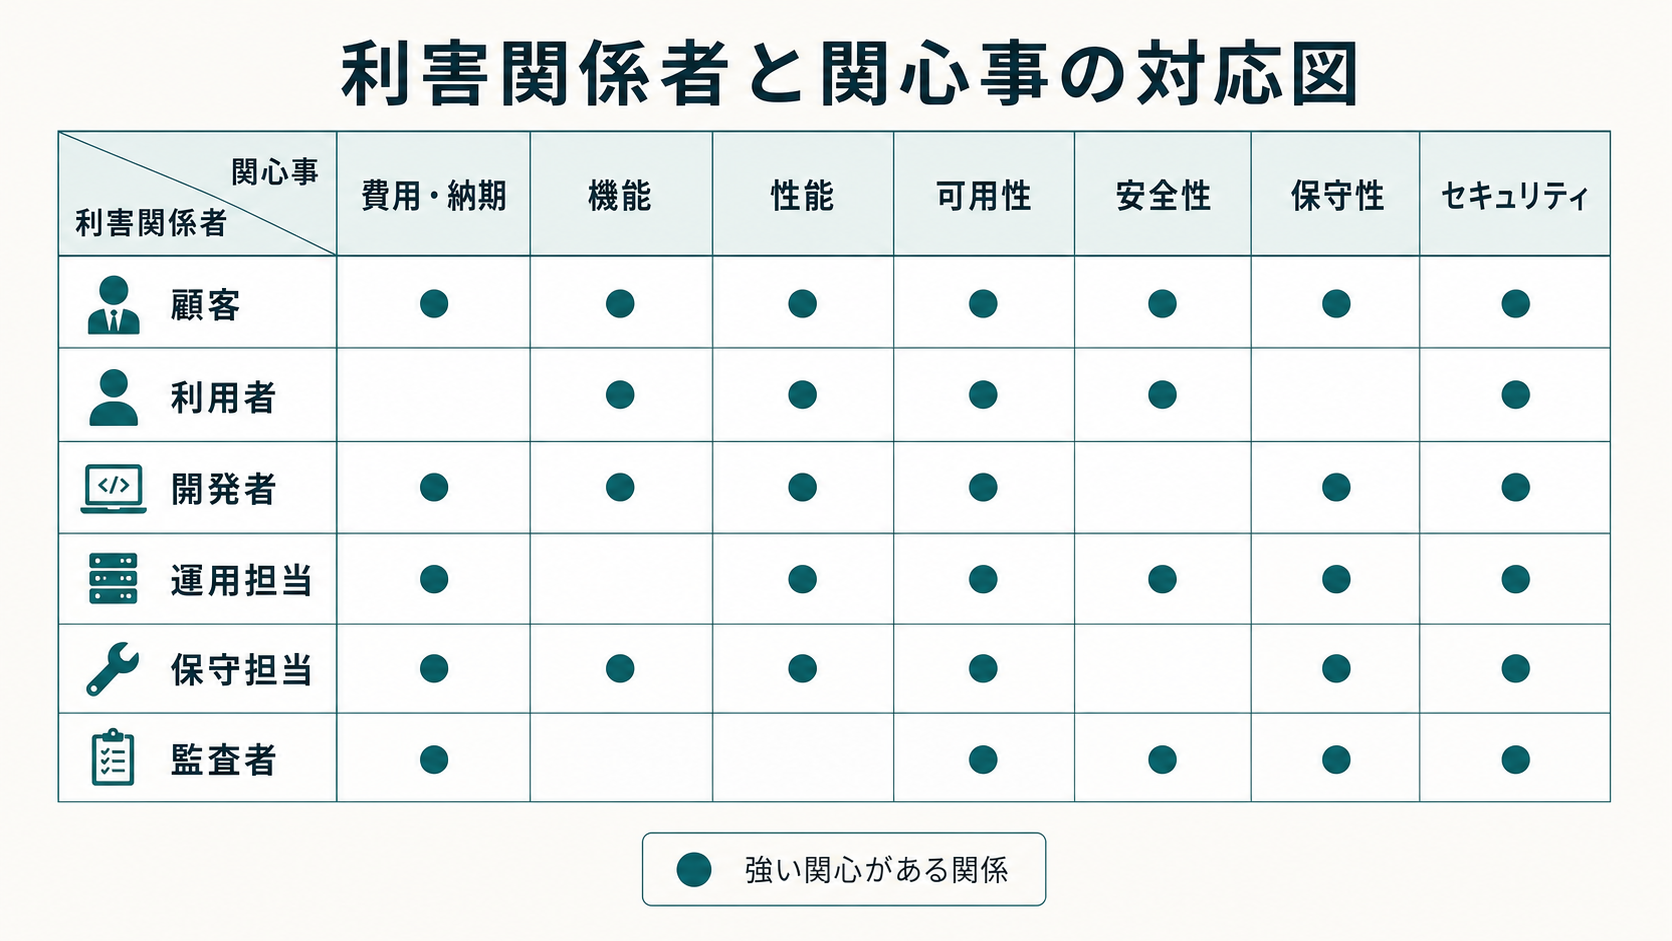
\includegraphics[width=0.96\linewidth]{assets/generated_figures/ch02/fig-ch02-03.png}}{\fbox{\parbox[c][48mm][c]{0.9\linewidth}{\centering 画像生成待ち\\利害関係者と関心事の対応図}}}
\caption{利害関係者と関心事の対応図}
\label{fig:ch02-03}
\end{figure}
